\chapter{Explicitly Correlated Methods}
\label{chap:explicit}

With the advent of modern computers combined with a vast array of sophisticated algorithms from which to choose, \emph{ab initio} quantum chemistry has become a tremendously powerful tool, going beyond the study of small atoms, to molecules and solids, and are among the most effective and systematically improvable techniques to date. Nevertheless, convergence to the \gls{CBS} limit is notoriously slow.

In particular, consider the popular basis set family developed by Dunning and coworkers, \gls{cc-pV$X$Z}.\cite{dunningGaussian1989a,woonGaussian1993,woonGaussian1994,petersonBenchmark1994,wilsonGaussian1996}
The size of these basis sets scale as $M\in\mathcal{O}(X^3)$, and since for standard post-Hartree-Fock discussed in chapter \ref{sec:post-hf} we require four-index integrals, our computation time will scale at least as $t\in\mathcal{O}(X^{12})$.\cite{klopperR122007}

Meanwhile, the \gls{CBS} correlation error scales as $\epsilon\in\mathcal{O}(X^{-3})$ \cite{helgakerBasisset1997,halkierBasisset1998} or $\epsilon\in\mathcal{O}(M^{-1})$,\cite{klopperInitio1995} resulting in $t\in\mathcal{O}(M^{-\frac 14})$. Thus, the methods discussed so far come with the painful cost of requiring very large basis sets to approach high-accuracy results.

Explicitly correlated methods are a class of electronic structure methods specifically designed to address this unfavourable scaling by explicitly including the interelectronic distance $r_{12}$, and is the subject of this chapter. As the R12/F12 family of methods is the most mature of the explicitly correlated electronic structure methods, many reviews focusing on this topic already exist. This chapter in particular is in large part based on three reviews: references \citenum{klopperR122007}, \citenum{gruneisPerspective2017} and \citenum{hattigExplicitly2012}.


\section{The Cusp Conditions}
\label{sec:cusp}

Consider two charged point particles in a system described by the Hamiltonian of equation \eqref{eq:elec_hamiltonian_2q}. By the Schr\"odinger equation, the local energy
\begin{equation}
    E_L\mathdef \frac{H\Psi}{\Psi}
\end{equation}
must be constant in the exact solution. However, when these two particles coalesce, i.e. $r_{12}\to 0$, the Coulomb potential, $r^{-1}$, diverges. Thus, for the local energy to be constant, we must have that near coalescence points, the kinetic energy exactly cancels the Coulomb energy. A more formal treatment of this argument leads to the electron-electron Kato cusp condition,\cite{katoEigenfunctionsManyparticleSystems1957a}
\begin{equation}
    \label{eq:cusp}
    \left.\widetilde{\frac{\partial \Psi}{\partial r_{12}}}\right|_{r_{12}\to 0}
    = \frac 12 \Psi(r_{12}=0)
\end{equation}
where the tilde represents spherical averaging.

This cusp condition was also later generalised.\cite{packCuspConditionsMolecular1966,kurokawaChapterTwoGeneral2016}
Early literature on the subject suggested that the success of explicitly correlated methods were due to the superior description of short-range correlation effects, and in particular in their much more faithful capturing of the cusp conditions like equation \ref{sec:cusp}.\cite{roothaanAnalytical1960,watsonApproximate1960,weissConfiguration1961,schwartzGround1962}
However, further study found that the correlation error from a bad description of the wave function around a small sphere centred on the cusp is actually negligible.\cite{coulsonElectron1961,gilbertInterpretation1963,prendergastImpact2001,klopperR122007} Instead, the success of explicitly correlated methods is actually due to the superior description of the overall shape and size of the Coulomb hole, which has a radius on the order of the atomic radius.

To understand why gaussian-type basis sets fail so spectacularly at capturing the cusp behaviour, it is instructive to consider a simpler example, like that of approximating $|x|$ by its Fourier decomposition. Such an illustration is found in figure \ref{fig:cusp}. It is also worth noting that \glspl{STO} do not suffer as badly from this limitation\cite{kongExplicitly2012}, but as discussed in chapter \ref{sec:orbitals}, they are unsuccessful due to their lack of practicality.

% \todo{would be nice to think of other ways to add images}

\begin{figure}[htbp]
    \centering
    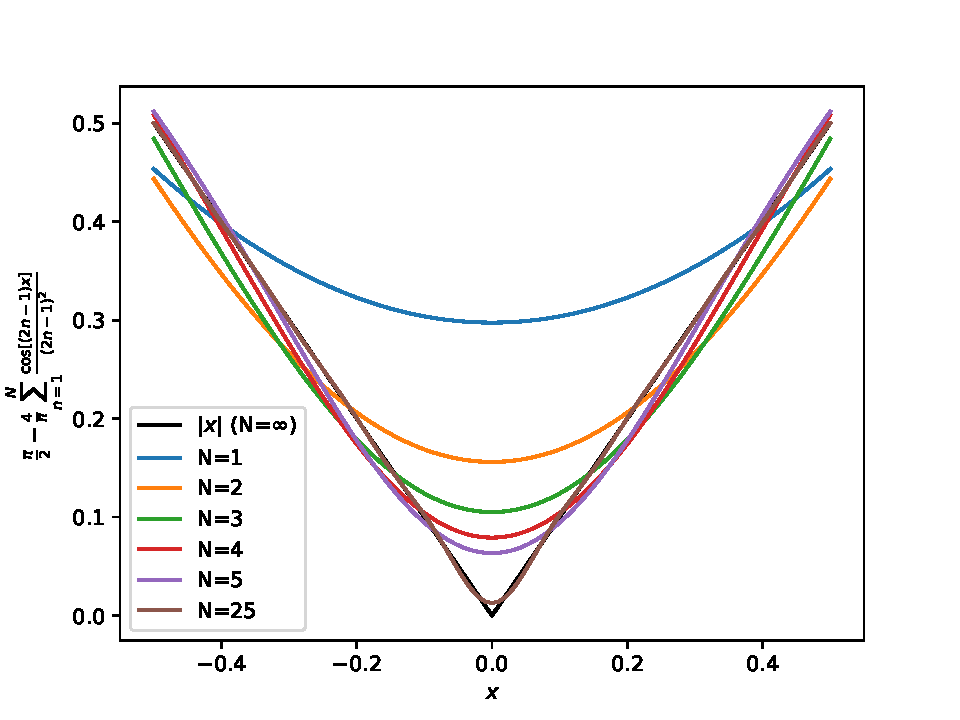
\includegraphics{figures/explicit/cusp.pdf}
    \caption{A toy example of the Coulomb cusp. Here, the Fourier expansion $x\approx\frac{\pi}{2} - \frac {4}{\pi} \sum_{n=1}^N\frac{\cos[(2n-1)x]}{(2n-1)^2}$ is plotted for a few values of $N$, including the exact solution. As can be seen, even for many terms, the Fourier expansion is a poor descripter in the cusp region. Indeed, the only way to describe it exactly is with an infinite number of terms.}
    \label{fig:cusp}
\end{figure}

\section{Hylleraas Methods}

Almost 30 years prior to Kato's landmark paper describing cusps in the analytical form for the wave function, there was already work being done to understand the significance of including $r_{12}$ in the wave function. Instead of being motivated by rigorous mathematics like Kato's, Slater was motivated by studyies in the He atom. In particular, he tried to construct a wave function which faithfully represents both the core region as well as the Rydberg limit (i.e. a highly excited atom where the electron is very far from the nucleus).\cite{kongExplicitly2012,grynbergIntroduction2010,slaterCentralFieldsRydberg1928,slaterNormal1928} This led him to suggest multiplying the wave function by a factor
\begin{equation}
    \e^{-2(r_1+r_2)+r_{12}/2},
\end{equation}
which can easily be shown to satisfy the cusp equation \eqref{eq:cusp}.

However, the first successful explicitly correlated electronic structure calculation is typically attributed to Hylleraas,\cite{hattigExplicitly2012}, where he aimed to improve convergence of orbital expansions for helium.\cite{hylleraasUeber1928,hylleraasNeueBerechnungEnergie1929} In this method, the coordinates $s\mathdef r_1+r_2$, $t\mathdef r_1 - r_2$ and $u\mathdef r_{12}$ are used to construct the wave function
\begin{equation}
    \Psi_N(s,t,u) = \e^{-\alpha s}\sum_{k}^N c_ks^{l_k}t^{2m_k}u^{n_k}.
\end{equation}

In particular, using only three terms ($N=3$), and variationally optimising for the parameters $c_1,c_2,c_3$, Hylleraas was able to reach within 1.3 millihartree from the exact result.

Since then, there was rapid development on this approach and combining it with \gls{CI} (which came to be known as the CI-Hyl methods).
\cite{largo-cabrerizoHylleraasCI1987,jamesGround1933,kolosAccurate1964,perkinsAtomic1968,perkinsAtomic1969,simsCombined1971,simsOneCenter1971,claryHylleraastype1977,claryCIHylleraas1976} In CI-Hyl methods, the wave function is expanded as in \gls{CI},
\begin{equation}
    \Psi = \sum_k c_k \Phi_k
\end{equation}
where
\begin{equation}
    \Phi_k = \mathcal{A} r^{\nu_k}_{ij}\prod_i\chi_{k_i}(\bm x_i)
\end{equation}
where ${\chi_k}$ is a spin-orbital basis and $\mathcal{A}$ is the antisymmetriser operator.

However, CI-Hyl methods were to eventually fall out of favour. This is because the expansions involve exceedingly difficult integrals involving many electrons and over products of correlation factors. This significantly restricts the tractibility and scalability of the method, and it has since largely gone unused.

\section{Explicitly Correlated Gaussians}

Boys\cite{boysIntegral1960} and Singer\cite{singerUse1960} independently introduced gaussian basis functions with explicit correlation for calculations on molecules. Much like how gaussian basis functions approximately

\todo{}
% \todo{see Kong reviews}
\gls{ECG} method developed by Boys and Singer\cite{boysIntegral1960,singerUse1960} (basis with explicit correlation baked in) $r_{ij}^\nu$ replaced by $\exp(-cr_{ij})$.
One major strength of this approach is that all integrals have closed-form algebraic expressions.\cite{lesterGaussian1964} Later, two-electron correlators, called \gls{GTG} were developed. review article \cite{mitroyTheory2013} Approximate linear r12 by combination of GTGs, avoid nonlinear optimisation \cite{bukowskiNew1994,perssonAccurate1996}

MP2\cite{panGaussian1970,panElectron1972}


approaches to avoid difficult integrals\cite{szalewiczNew1982,szalewiczAtomic1983,wenzelAtomic1986,szalewiczAtomic1984,tewWeak2007}

\todo{}

While not as popular as F12 methods (see section \autoref{sec:f12}), \glspl{ECG} have been used for highly accurate variational calculations\cite{korobovCoulomb2000}, as well as for applications outside of standard electron structure theory, such as bosons\cite{vargaPrecise1995}, positronium (a bound state of electron and positron)\cite{bubinGroundstate2011}, and non-Born-Oppenheimer systems\cite{stankeNonBornOppenheimer2009}.

\section{F12 Methods}
\label{sec:f12}

\subsection{A Historial Perspective: R12 Methods}
\todo{... see review papers haettig pg 30 for basic intro then 35 - 50 then excited state papers}

\todo{revisit}
brief mention of how it builds on gaussian-type geminals

\subsection{}

\todo{make sure to include some excited state information}

\section{The Transcorrelated Method}
\label{sec:tc}
\todo{brief recap of Boys-Handy method, some extensions by other people, and how it is used in our group}

Hirschfelder first introduced a similarity transform method \cite{hirschfelderRemoval1963}

then was worked on by Boys and Handy \todo{cite}, to be discussed here

recent renewal of interest (lots and lots of citations) with various applications, including DMRG, quantum computing, etc.

will talk in more detail about the Jastrow factor in section \ref{sec:jastrow} since it is also used in vmc

\todo{also mention biorthogonal orbitals etc.}

\subsection{The Method of Boys and Handy}

\subsection{Modern Resurgence}
\todo{Also cite Werner and quantum computing people}


\subsection{Comparison to F12/R12}

discuss additive vs multiplicative ansatz

have some performance comparison plots, maybe can ask permission to reproduce from Evelin or someone else

also discuss many-body integrals for f12 vs at most 3-body for tc


\todo{Maybe have a picture of basis set convergence? Maybe even just HF, compare F12 vs TC vs Hyl(?) vs standard}
